\documentclass[11pt,a4paper]{article}

\usepackage[polish]{babel}
\usepackage[utf8]{inputenc}
\usepackage{polski}
\usepackage[T1]{fontenc}
\usepackage{indentfirst}
\usepackage{wrapfig}    % for wrapping figures, tables

\frenchspacing

%\usepackage{amsmath}
\usepackage{physics}
%\usepackage{bm}
\usepackage{gensymb}
%\usepackage{hepnames}
\usepackage{epsfig}
\usepackage{graphics}
\usepackage[shortlabels]{enumitem}
%\usepackage{xspace}
%\xspaceaddexceptions{[]\{\}}

%
%
%fixpagesize
\pagestyle{empty}
\addtolength{\textwidth}{6cm}
\addtolength{\textheight}{4cm}
\addtolength{\evensidemargin}{-3cm}
\addtolength{\oddsidemargin}{-3cm}
\addtolength{\topmargin}{-2cm}
\parindent=0cm


%
%
%small distance in list/item/enum for enumitem package
\setlist[itemize,enumerate]{topsep=0em}
\setlist{noitemsep}

%print zadanie #
\newcounter{zadanie}\newcommand{\zadanie}[1][]{\addtocounter{zadanie}{1} ~\\  {\bf \emph{Zadanie \arabic{zadanie} #1 }} \\}
\newcounter{zaddom}\newcommand{\zaddom}[1][]{\addtocounter{zaddom}{1} ~\\  {\bf \emph{Zadanie domowe \arabic{zaddom} #1 }} \\}
%\renewcommand{\zadanie}[1][]{\pagebreak  ~\\  {\bf \emph{Zadanie }} \\} \addtolength{\topmargin}{-2cm}

\newcommand{\dbar}{{\mkern3mu\mathchar'26\mkern-12mu d}}


%%%%%%%%%%%%%%%%%%%%%%%%%%%%%%%%%%%%%%%%%%%%%%%%%%%%%%

\begin{document}           % End of preamble and beginning of text.

\begin{centering}
\bf{\Large{Termodynamika z elementami fizyki statystycznej}}\\
Tydzień 11 (19 maja 2023)\\[0mm]
Kombinatoryka, mikrostany, entropia układu izolowanego\\
\end{centering} 
\vspace{5mm}

\zadanie
Gęstość rozkładu prawdopodobieństwa masy truskawek z transportu jest zadana wzorem:\\
$dN = A \cdot m^2 \cdot \exp(-m/M) \cdot dm = f(m) \cdot dm$, gdzie parametr $M = 30\,$g.
\begin{enumerate}[a)]
\item Wyznacz stałą $A$.
\item Gdzie leży maksimum rozkładu $f(m)$? Jaka jest średnia waga truskawki?
\item Kontrahent potrzebuje truskawek o masach zawartych pomiędzy 27\,g a 33\,g. Jaki procent truskawek możemy mu sprzedać?
Oszacować wynik jako $f(m)\cdot \Delta m$ i porównać z wynikiem dokładnym otrzymanym przez całkowanie $f(m)$.
\end{enumerate}
Pomocnicza całka
\[
\int_0^\infty x^n e^{-ax}dx=n!/a^{n+1}
\]

\vspace{0.5cm}
{\bf \em Rozwiązanie:} Normalizacja:
\[
1= \int_0^{\infty} f(m)\mathrm{d}m= 2A\,M^3
\]
czyli $A=1/(2M^3)$.

Maksimum, z warunku $f'(m)=0$ jest dla $m=M$.\\

Średnia masa truskawki to:
\[
\int_0^{\infty} m f(m)\,\mathrm{d}m= 3M
\]

Udział truskawek w pożądanym zakresie mas to:
\[
\frac{1}{2\,30^3}\int_{27}^{33}m^2e^{-m/30}dm/2\cdot\simeq 0.0367
\]

\begin{wrapfigure}[7]{r}{0.15\linewidth}\vspace{0mm}
\resizebox{\linewidth}{!}{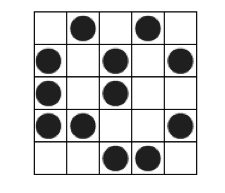
\includegraphics{tydzien10_rys1.png}}
\end{wrapfigure}
\zadanie
Znaleźć liczbę mikrostanów w układzie układu $N$ nierozróżnialnych kulek rozmieszczonych w pudełku z $V$ przegródkami ($V$ oraz $N$ definiują makrostan układu). Wykonać obliczenia dla $V = 20$ i $N = 10$ za pomocą ścisłego wzoru oraz przybliżając wynik używając wzór Stirlinga: $\displaystyle n! \approx \sqrt{2 \pi n} \left(\frac{n}{e}\right)^n$.
\vspace{5mm}

{\bf \em Rozwiązanie:} Liczba kombinacji czyli na ile sposobów można wybrać pozdbiór $N$ elementowy w $V$-elementowym
\[
\binom{V}{N}=\frac{V!}{N!(V-N)!}=184756
\]
Ze wzorzu Stirlinga:
\[
\binom{V}{N}=\frac{1}{\sqrt{2\pi}}\sqrt{\frac{20}{10^2}}\frac{20^{20}}{10^{20}}=187078.97
\]

\zadanie
Rozważyć układy $N$ niezależnych cząstek:\begin{enumerate}[a)]
\item klasycznych,
\item kwantowych o spinie całkowitym (tj. bozonów),
\item kwantowych o spinie połówkowym (tj. fermionów).
\end{enumerate}
Zakładając, że pojedyncza cząstka może przebywać w $R$ stanach jednocząstkowych, obliczyć ile wynosi liczba mikrostanów każdego z wymienionych układów.

{\bf \em Rozwiązanie:} Klasycznie, cząstki są rozróżnialne, każda niezależnie zajmuje jeden z $R$ stanow czyli łącznie $R^N$. Bozony mogą zajmować te same stany i są nierozróżnialne.
Najprościej uszeregować cząstki (kulki) i granice kolejnych stanów (kreski), jak na rysunku.
Wtedy wybieramy pozycje $N$ kulek na $N+R-1$ możliwości (jednej kreski nie ma bo są ściany).
Na rysunku pokazany jest przypadek $N=9$ i $R=8$ (czyli $7$ kresek). Stany są jednoznacznie obsadzone przez kolejne liczby kulek $1,2,0,1,3,2,0,0$.
\begin{center}
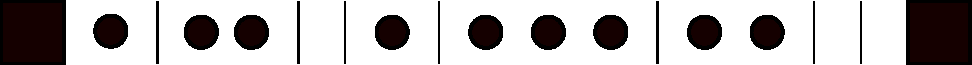
\includegraphics[width = 0.7\linewidth]{kulkres.pdf}
\end{center}
Daje to liczbę stanów:
\[
\binom{N+R-1}{N}
\]

Fermiony mogą obsadzać stany jednocząstkowe pojedynczo, a liczba konfiguracji to:
\[
\binom{R}{N}
\]


\zadanie
Rozważyć układ składający się z dwóch odizolowanych od siebie części: $A$ oraz $B$, 
z których każda zawiera dwie rozróżnialne cząstki mogące przebywać w dyskretnych
stanach energetycznych o energiach będących całkowitą wielokrotnością $\varepsilon$. 
Niech energie podukładów wynoszą odpowiednio $E_A = 5\,\varepsilon$ i $E_B = \varepsilon$. 
\begin{enumerate}[a)]
\item 
Obliczyć ile wynosi liczba mikrostanów $\Omega_{A \cdot B}$ opisanego układu.
\item Jaka będzie liczba mikrostanów $\Omega_{A+B}$ tego układu, jeśli dopuścimy swobodny przepływ
energii pomiędzy podukładami $A$ i $B$ (tzn. usuniemy adiabatyczną przegrodę pomiędzy podukładami)?
\item Przyjmując postulat, że w równowadze termodynamicznej 
wszystkie mikrostany realizujące dany makrostan układu izolowanego są jednakowo
prawdopodobne, obliczyć jakie jest prawdopodobieństwo, że po usunięciu przegrody
energia podukładu $A$ wzrośnie?
\item Jaki podział energii między podukładami $A$ i $B$ jest najbardziej prawdopodobny (tzn. odpowiada stanowi równowagi układu $A + B$)?
\end{enumerate}

{\bf \em Rozwiązanie:} $E_A=q_A\epsilon$, $E_B=q_B\epsilon$, $q_A=q_{A1}+q_{A2}$, $q_B=q_{B1}+q_{B2}$
$q_{A12,B12}\geq 0$ dla całkowitych $q$.

Wtedy $\Omega_A=6$, $\Omega_B=2$, czyli $\Omega_{A \cdot B}=6\cdot 2=12$.
Do obliczenia $\Omega_{A+B}$ zakładamy dowolne stany relaizujące $q=q_A+q_B=6$. Jest to taka sam sytacja jak w zad 3b, dla $N=q$ i $R=4$ 
czyli $\Omega_{A+B}=84$. Prawdopodobieństwo $q_A=6$ wynosi $7/84=1/12$ bo $7$ stanów daje $E_A=6$, w wszystkie są równie prawdopodobne.
Najbardziej prawdopodobne jest $q_A=3$ bo liczba stanów jest $4\cdot 4=16$, czyli $p=16/84=1/3$. Dla porównania $p(q_A=2)=p(q_A=4)=5\cdot 3/84=5/28$
oraz $p(q_A=1)=p(q_A=5)=6\cdot 2/84=1/7$ a $p(q_A=6)=p(q_A=0)=7/84=1/12$
Entropia $S=k\ln\Omega$ gdzie $k$ -- stała Boltzmanna.

\zadanie
{\em Model Einsteina drgań sieci krystalicznej ciał stałych  (model nieoddziałujących oscylatorów)}\\
Rozważyć układ $N$ rozróżnialnych cząstek, z których każda może przebywać w dyskretnych stanach energetycznych o energiach będących całkowitą wielokrotnością pewnego $\varepsilon$ (tzn. $0,\,\varepsilon,\,2\,\varepsilon,\,3\,\varepsilon$, etc.) --- czyli że są one kwantowymi oscylatorami harmonicznymi. Wyprowadzić wzór na liczbę możliwych stanów (mikrostanow) $\Omega (N, q)$ tego układu realizujących warunek, że całkowita energia układu wynosi $E = q\cdot\varepsilon$. 
Wykonaj przybliżone obliczenia dla $N = 30$ i $q = 30$ przy zastosowaniu wzoru Stirlinga i podaj entropię układu.
\vspace{5mm}

{\bf \em Rozwiązanie:} Liczymy jak w zad 3b, zamieniając $N\to R$ $q\to N$ tj.
\[
\Omega=\binom{N+q-1}{q}
\]
W przybliżeniu:
\[
S=k\ln\Omega\simeq k[(N+q-1)ln(N+q-1)- q\ln q-(N-1)\ln(N-1)]
\]

\zadanie
Rozważyć dwa mogące wymieniać energię układy zawierające $N$ cząstek każdy: $N_A = N_B = N$, 
o całkowitej energii równej $q_A\cdot\varepsilon + q_B\cdot\varepsilon = q\cdot\varepsilon$ (gdzie $\varepsilon$ jest pewnym kwantem energii). 
Stosując model nieoddziałujących oscylatorów oraz zakładając że energia obu podukladów jest duża ($q_i \gg N$), pokazać, że:
\begin{enumerate}[a)]
\item całkowita liczba mikrostanów układu 
      $\Omega_{tot} = \Omega_A \cdot \Omega_B$  
      ma maksimum dla $\displaystyle q_A = q_B = q/2$,
\item $\Omega_{tot}$ w okolicy swego maksimum jest funkcją Gaussa parametru 
      $x$ (gdzie: $\displaystyle q_A = \frac{q}{2} + x$ oraz\linebreak 
      $\displaystyle q_B = \frac{q}{2} - x$),
      której względna szerokość jest rzędu $1/\sqrt{N}$.
\end{enumerate}

{\bf \em Rozwiązanie:} Jak w poprzednim zadaniu

\[
\Omega_A=\binom{N+q_A-1}{q_A},\;\Omega_B=\binom{N+q_B-1}{q_B}
\]
Zauważmy że $\Omega_A\Omega_B$ zwiększa się gdzy wyrównujemy $q$
dla $q'_A=q_A+1$, $q'_B=q_B-1$ oraz $q'_B\geq q_A$ (co jednocześnie oznacza $q_B\geq q'_A$)
mamy
\[
\Omega'_A\Omega'_B=\Omega_A\Omega_B\frac{(N+q_A)q_B}{(N+q'_B)q'_A}\geq \Omega_A\Omega_B
\]
bo 
\[
\frac{N-1}{q'_A}\geq \frac{N-1}{q_B}
\] 
skąd po dodaniu $1$ do obu stron
\[
\frac{N+q_A}{q'_A}\geq\frac{N+q'_B}{q_B}
\]
Podobnie, stosując wzór Stirlinga
\[
\ln\Omega_{tot}=(N-1+q/2+x)\ln(N-1+q/2+x)+(N-1+q/2-x)\ln(N-1+q/2-x)
\]
\[
-(q/2+x)\ln(q/2+x)-(q/2-x)\ln(q/2-x)+C
\]
gdzie $C$ jest stałą.
Zakładając małe $x$, rozwijając $(y+x)\ln(y+x)\simeq y\ln y+x(1\ln y)-x^2/2y$ dla małych $x$ otrzymamy
\[
\ln\Omega_{tot}\simeq C-2x^2/q+2x^2/(2N-2+q)\simeq C-4x^2(N-1)/q^2
\]
dla $N\ll q$. Wariancja $\langle\langle x^2\rangle\rangle\sim q^2/8N$

\vspace*{1cm}

\begin{wrapfigure}[7]{r}{0.3\linewidth}\vspace{-3mm}
\resizebox{\linewidth}{!}{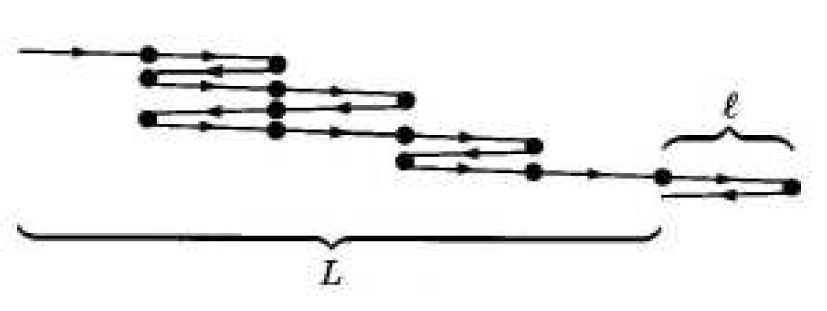
\includegraphics{tydzien10_rys2.png}}
\end{wrapfigure}
\zaddom
Obliczyć entropię jednowymiarowego łańcucha przedstawionego na rysunku, przy założeniu,
że składa się on z $N$ elementów ($N\gg 1$) o długości $\ell$ każdy. 
Przyjąć, że odległość pomiędzy początkowym i
końcowym punktem tego łańcucha wynosi $L$.\\
{\bf \em Odpowiedź:} $S=k(\log N!-\log N_+!-\log N_-!)$

\zaddom
Rozpatrz dwa izolowane układy rozróżnialnych, nieruchomych i nieoddziałujących cząstek. Każda cząstka znajduje się w jednym z trzech stanów o energiach:
$-\varepsilon$, 0, $\varepsilon$.
Pierwszy układ (układ {\bf A}) zawiera jedną cząstkę, a jego całkowita
energia wynosi $E_A = \varepsilon$.
Drugi układ (układ {\bf B}) zawiera trzy cząstki, a jego całkowita
energia wynosi $E_B = -\varepsilon$.
\begin{enumerate}[(a)]
\item   Policz liczbę mikrostanów całości złożonej z obu izolowanych układów.
\item   Układy doprowadzono do kontaktu ze sobą tak, że mogą one wymieniać energię.
            Jaka jest teraz liczba mikrostanów?
\item   Ile wynosi teraz najbardziej prawdopodobna energia układu {\bf A}?
\item   Ile wynosi entropia całego układu w punktach a) i b)\,?
\end{enumerate}
{\bf \em Odpowiedź:}  a) $\Omega_A=1$, $\Omega_B=6$, ~~ b) $\Omega=19$, ~~ c)   $0$, $S=k\log\Omega$.

\zaddom
Energia wewnętrzna układu $N$ atomów tworzących $N$-punktową idealną sieć krystaliczną wynosi $U_0$.
Atomy mogą jednak zajmować także miejsca pomiędzy punktami sieci (defekt sieci, takich miejsc dyslokacji też jest $N$).
Atom znajdujący się poza punktami sieci ma dodatkową energię $\epsilon$ i może z równym prawdopodobieństwem wybrać każdy niezajęty punkt dyslokacji.
Znajdź entropię układu, jeżeli jego energia wewnętrzna wynosi $U_0 + n\epsilon$.\\
{\bf \em Odpowiedź:} Liczba kombinacji bez powtórzeń $\left( \begin{tabular}{c}  N \\ $n$\end{tabular} \right)$.


% An example of figure placement:
%\begin{wrapfigure}[13]{r}{0.4\linewidth}\vspace{3mm}
%\resizebox{\linewidth}{!}{\includegraphics{NAZWA.png}}
%\end{wrapfigure}
%\zadanie

\end{document}
